\documentclass[aspectratio=1610]{beamer}

\usetheme{metropolis}

\usepackage[russian]{babel}
\usepackage{polyglossia}
\setdefaultlanguage{russian}
\setmainfont{Arial}
\setromanfont{Times New Roman}
\setsansfont{Arial}
\setmonofont{Courier New}

\usepackage{fontspec}
\setmainfont{Times New Roman}
\newfontfamily{\cyrillicfont}{Times New Roman}
\newfontfamily{\cyrillicfontrm}{Times New Roman}
\newfontfamily{\cyrillicfontsf}{Arial}
\newfontfamily{\cyrillicfonttt}{Courier New}

\usepackage{minted}
\setminted{fontsize=\small,baselinestretch=1}

\usepackage{graphicx}
\graphicspath{{../pictures/}}
\DeclareGraphicsExtensions{.pdf,.png,.jpg}

\usepackage{tikz}
\usetikzlibrary{automata,arrows,chains,shapes.geometric,positioning,calc}

\title[Thesis]{Исследование возможности использования подмены библиотеки для реализация палитры команд}
\author{Студент: Польшаков Д.В. \\ Научный руководитель: Чернышов М.К.}
\institute{ВГУ}
\date{\the\year}

\begin{document}
	
\frame{\titlepage}

\begin{frame}{Палитра команд}
	Это специальное окно в интерфейсе приложения, где отображаются все доступные
	функции. Иногда рядом с описанием функции отображается горячая клавиша для
	её активации.
\end{frame}

\begin{frame}{Палитра команд в VS Code}
	\centering
	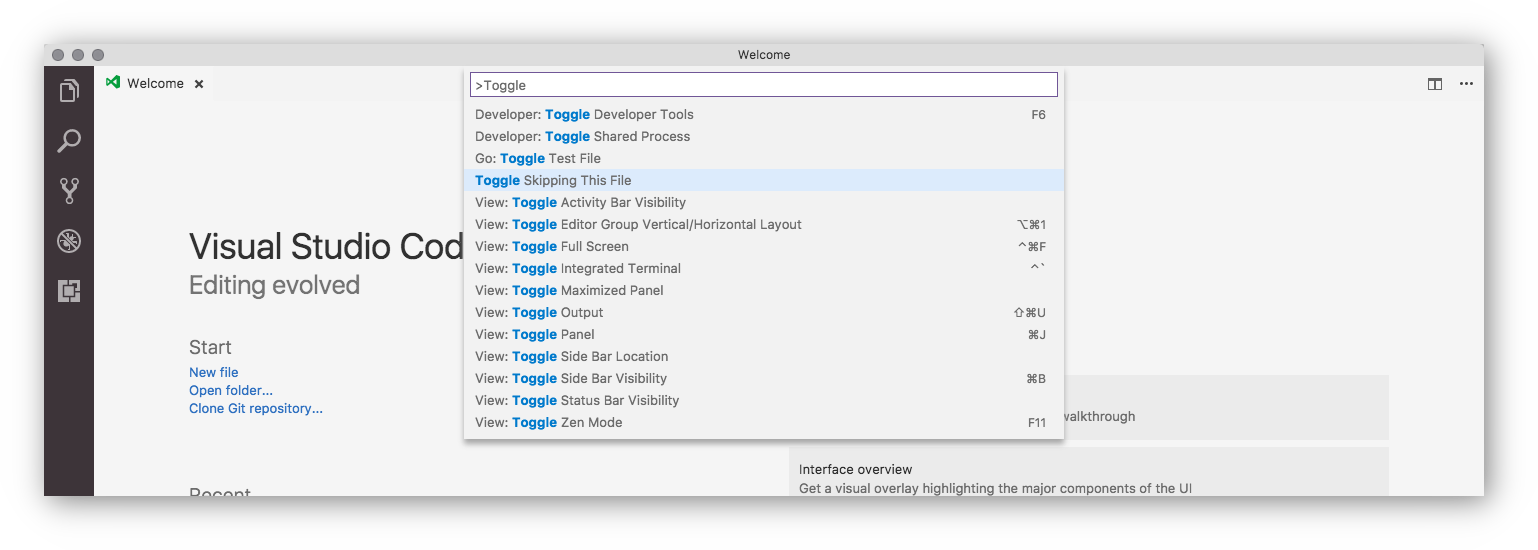
\includegraphics[width=\textwidth]{vscode}
\end{frame}

\begin{frame}{Палитра команд в Plotinus}
	\centering
	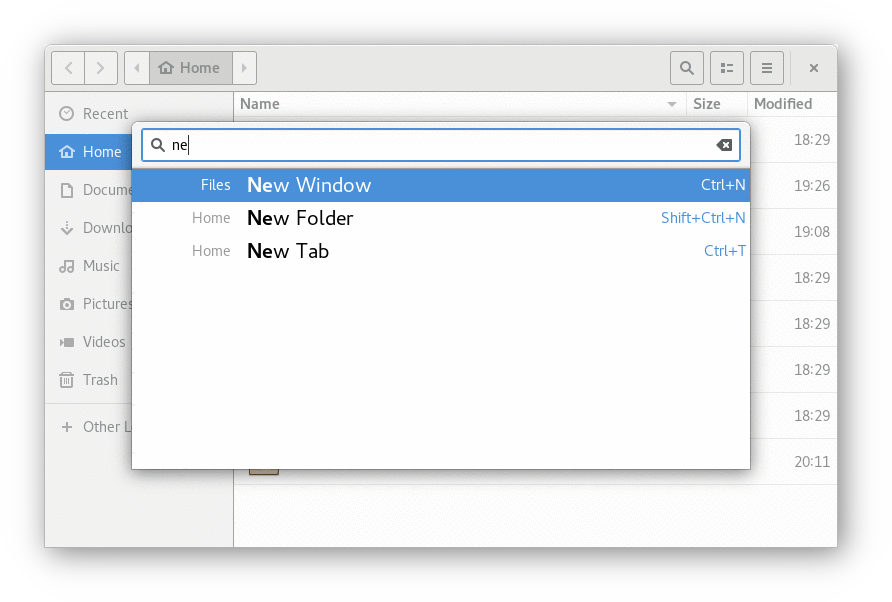
\includegraphics[height=0.9\textheight]{Plotinus}
\end{frame}

\begin{frame}{Qt}
    \begin{columns}
		\column{0.38\linewidth}
		\centering
		
\includegraphics[width=5cm]{Qt}
		\column{0.58\linewidth}
		\textbf{Qt}~— кроссплатформенный фреймворк для разработки программного обеспечения на языке программирования C++. Включает в себя в т.ч. классы для разработки
		графического интерфейса.
	\end{columns}	
\end{frame}

\begin{frame}{Добавление логики в приложение}
	\textbf{Способы добавления дополнительной логики в приложение}
	\begin{itemize}
		\item добавление функции на этапе сборки приложения
		\item добавление функции в момент выполнения программы
		\begin{itemize}
			\item с помощью загрузка плагинов
			\item с помощью подмены библиотек
		\end{itemize}
	\end{itemize}
\end{frame}

\iffalse
\begin{frame}{Взаимодействие элементов GUI и пользователя}
	\begin{figure}
		\begin{tikzpicture}[
        ->,>=stealth',node
        distance=1.5cm, semithick,
        every edge/.append style={<->}
    ]

    \tikzstyle{block} = [rectangle,draw,minimum height=0.8cm]

    \node[block] (user) {Пользователь};
    \node[block] (x11) [below of=user] {Графическая подсистема X11};
    \node[block] (lib) [below of=x11] {Графическая библиотека Qt};
    \node[block] (app) [below of=lib] {Приложение};
    \path[]
        (user) edge (x11)
        (x11) edge (lib)
        (lib)  edge (app)
    ;

\end{tikzpicture}

	\end{figure}
\end{frame}
\fi

\begin{frame}{Постановка задачи}
	Разработать набор программ, которые в комплексе будут решать следующие
	задачи:
	
	\begin{itemize}
		\item запускать целевые приложения в специальном окружении
		\item собирать информацию о существующих элементах графического приложения
		\item сохранять информацию о всех запущенных приложениях
		\item отображать пользователю окно для поиска и выбора элемента
		\item активировать выбранный пользователем элемент
	\end{itemize}
\end{frame}

\begin{frame}{Постановка задачи}
	Набор программ должен быть реализован в виде следующих элементов:
	
	\begin{enumerate}
		\item\label{lib} Библиотека для внедрения и сбора информации в конкретном
		приложении.
		\item Приложение для сохранения информации, полученой из нескольких
		приложения с библиотекой из п.\ref{lib}.
		\item Графический интерфейс для запуска приложений и отображения окна
		палитры комманд.
	\end{enumerate}
\end{frame}

\iffalse
\begin{frame}{Общая архитектура}
	\centering
	\begin{tikzpicture}[
        ->,>=stealth',node
        distance=2cm, semithick
    ]

    \tikzstyle{block} = [rectangle,draw,minimum height=0.8cm]

    \node[block] (preload) {Подгружаемый модуль};
    \node[block] (lib)    [above of=preload] {libQtWidgets};
    \node[block] (x11)    [above of=lib]     {X11};
    \node[block] (server) [left=2cm of preload] {Сервер управления};
    \node[block] (app)    [below of=preload] {Целевое приложение};

    \node[block] (ctrl) [above of=server] {Приложение управления};
    \node[block] (user) [above of=ctrl] {Пользователь};

    \path[]
        (app)     edge[bend left]     node[left]  {1} (preload)
        (preload) edge[bend left=5]   node[below] {2} (server)
        (preload) edge[bend left]     node[left]  {3} (lib)
        (lib)     edge[bend left]     node[left]  {4} (x11)
        (server)  edge[bend left]     node[left]  {5} (ctrl)
        (ctrl)    edge[bend left]     node[left]  {6} (user)
        (user)    edge[bend left]     node[right] {7} (ctrl)
        (ctrl)    edge[bend left]     node[right] {8} (server)
        (server)  edge[bend left=5]   node[above] {9} (preload)

        (server.north east)  edge    node[above]{10} (x11)

        (x11)     edge[bend left]     node[right] {11} (lib)
        (lib)     edge[bend left]     node[right] {12} (preload)
        (preload) edge[bend left]     node[right] {13} (app)
        (preload) edge[bend right=75] node[right] {14} (lib)
        (lib)     edge[bend left=80]  node[right]  {15} (app)
    ;

\end{tikzpicture}

\end{frame}
\fi

\begin{frame}{Генерация кода}
	Искажение имен (name mangling):
	\begin{itemize}		
		\item \texttt{QCheckBox::QCheckBox(const QString\&, QWidget*)}
		\item \texttt{\_ZN9QCheckBoxC1ERK7QStringP7QWidget\_f}
		\item \texttt{void QAbstractButton::setText(const QString\&)}
		\item \texttt{\_ZN15QAbstractButton7setTextERK7QString\_f}
	\end{itemize}
\end{frame}

\begin{frame}[fragile]{Генерация кода}
	Однотипный код
	\begin{minted}{cpp}
    typedef bool *func_f(int a, char* s);
    static func_f real_func = 0;

    bool func(int a, char* s)
    {
        if (!real_func)
            real_func = (func_f)dlsym(RTLD_NEXT, "func");

        if (initInject())
            handle_for_func(a, s); // to change
            
        return real_func(a, s);
    }
	\end{minted}
\end{frame}

\begin{frame}[fragile]{Протокол}
	\begin{minted}{text}
    <команда> ::= <имя-­команды> <параметры-­команды>
    <имя-­команды> ::= <строка>
    <строка> ::= <длина-­строки> <идентификатор>
    <длина-­строки> ::= uint32_t
    <идентификатор> ::= "newApp"
                    ::= "setWidgetText"
                    ::= "remove"
                    ::= "activated"
                    ::= "setWidgetWindow"
                    ::= "activate"
	\end{minted}
\end{frame}

\iffalse
\begin{frame}{Приложение управления}
	\centering
	\input{../schemes/app_arch.tex}
\end{frame}
\fi

\begin{frame}{Интерфейс}
    \begin{columns}
		\column{0.58\linewidth}
		Сочетания клавиш
		\begin{itemize}
			\item Запуск: Ctrl + Shift + D
			\item Палитра: Ctrl + Shift + S
		\end{itemize}
		\column{0.38\linewidth}
		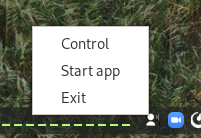
\includegraphics[width=3cm]{tray_ui}
	\end{columns} 
\end{frame}

\begin{frame}{Интерфейс}
    \begin{columns}
		\column{0.5\linewidth}
		\textbf{Запуск приложений}
		\centering
		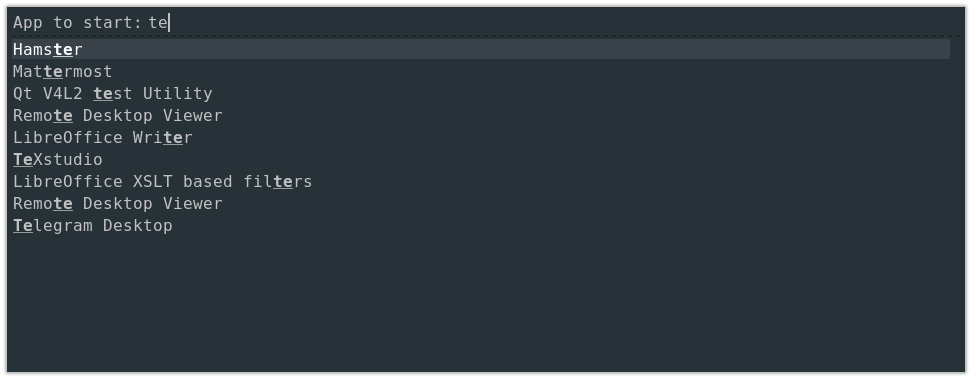
\includegraphics[width=\textwidth]{start_ui}
		\column{0.5\linewidth}
		\textbf{Палитра команд}
		\centering
		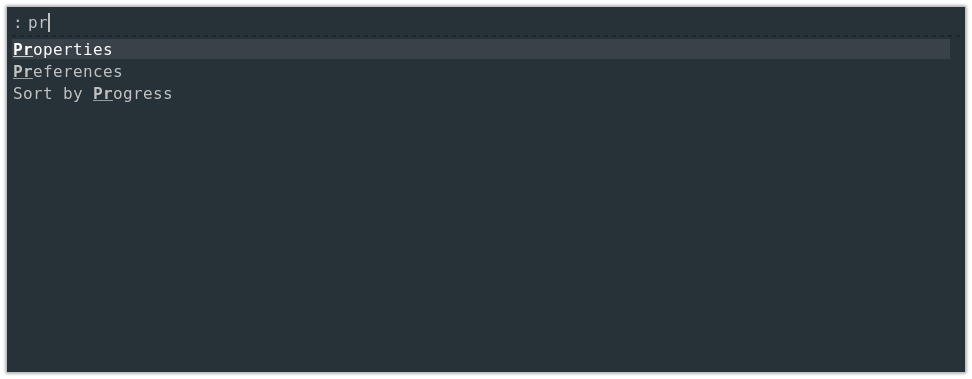
\includegraphics[width=\textwidth]{control_ui}
	\end{columns}
\end{frame}

\begin{frame}{Заключение}
	\begin{itemize}
		\item Реализована библиотека, для перехвата событий
		\item Реализован вспомогательный генератор для расширения библиотеки
		\item Разработано приложение для внедрения библиотеки и отображения палитры команд
	\end{itemize}
\end{frame}

\frame{\titlepage}

\end{document}